\documentclass{beamer}
\usepackage[utf8]{inputenc}
\inputencoding{latin1}
\usepackage[T1]{fontenc}
\usepackage[spanish,english]{babel}
\usepackage{graphics}
\usepackage{graphicx}
\usetheme[secheader=true]{Madrid}
\useinnertheme{rectangles}
\usepackage{tikz}
\title{FPGA \& DDR DRAM}
\author[msagre]{Miguel A Sagreras}
\date[2015]{}
%\institution[short name]{long name}
\begin{document}

\begin{frame}
\titlepage
\end{frame}

\section{Primeras computadoras}
\subsection{Tecnolog�a anal�gica}
\begin{frame}
\frametitle{Torpedo Data Computer}
\subsection{Electromec�nicas Anal�gicas}
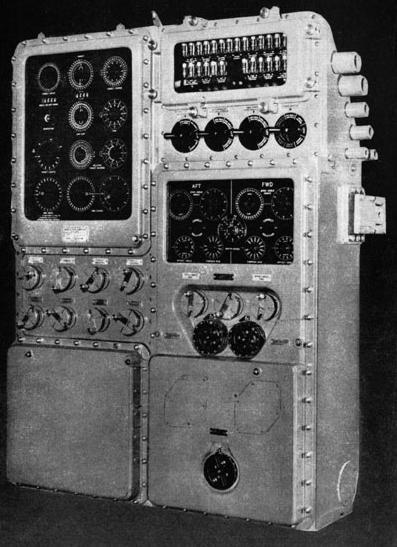
\includegraphics[width=3.2cm]{TDC-image.jpg} 

%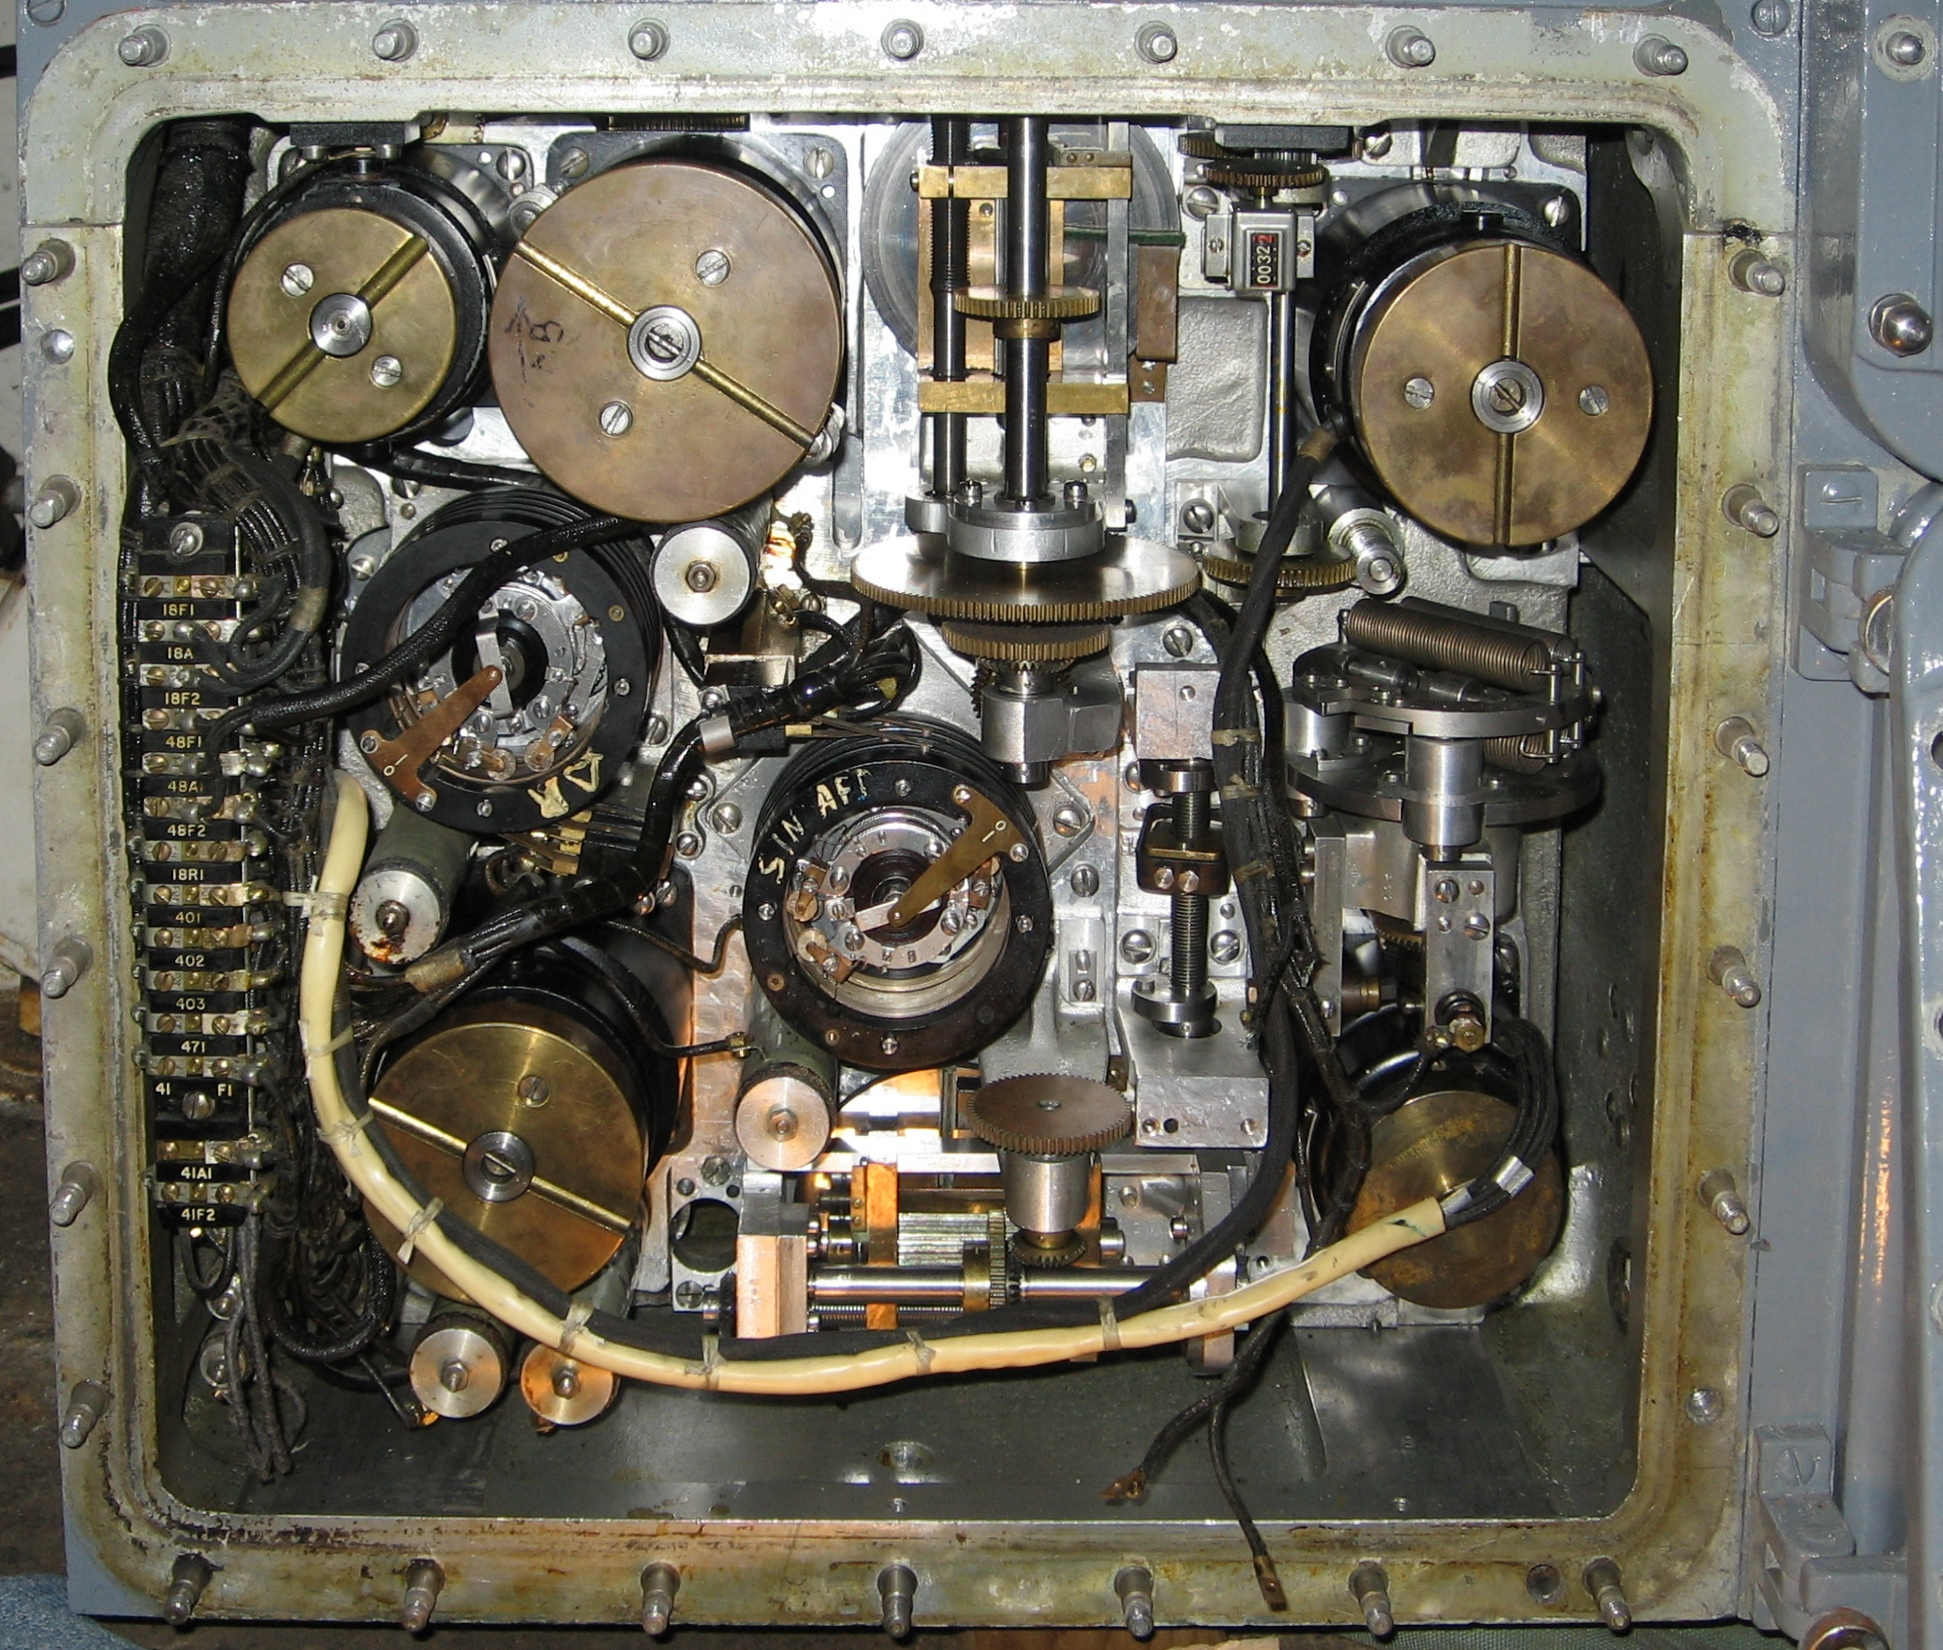
\includegraphics[width=3.2cm]{TDC-inside.jpg}
\end{frame}

\subsection{Tecnolog�a digital electromec�nica}

\begin{frame}
\frametitle{Relay}
\framesubtitle{Componente b�sico}
\begin{minipage}[c]{6cm}
	\begin{center}
		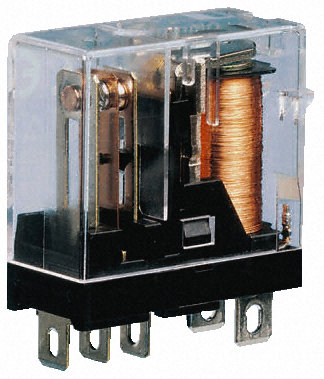
\includegraphics[height=3cm]{relay-imagen.jpg}
	\end{center}
\end{minipage}
\begin{minipage}[c]{5cm}
	\begin{center}
		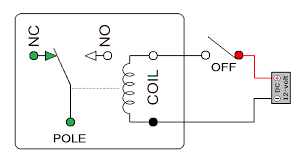
\includegraphics[height=3cm]{relay-diagrama.png}
	\end{center}
\end{minipage}
\end{frame}

\begin{frame}
\frametitle{Z3}
\begin{minipage}[c]{5.25cm}
	\begin{itemize}
		\item 1941
		\item Konrad Zuse
		\item Estudio de aeroelasticidad
		\item 64 palabras de 22 bits
		\item 5 Hz
		\item 2000 relays
		\item 4 KW
		\item 1 Tonelada
	\end{itemize}
\end{minipage}
	\begin{minipage}[c]{6.4cm}
		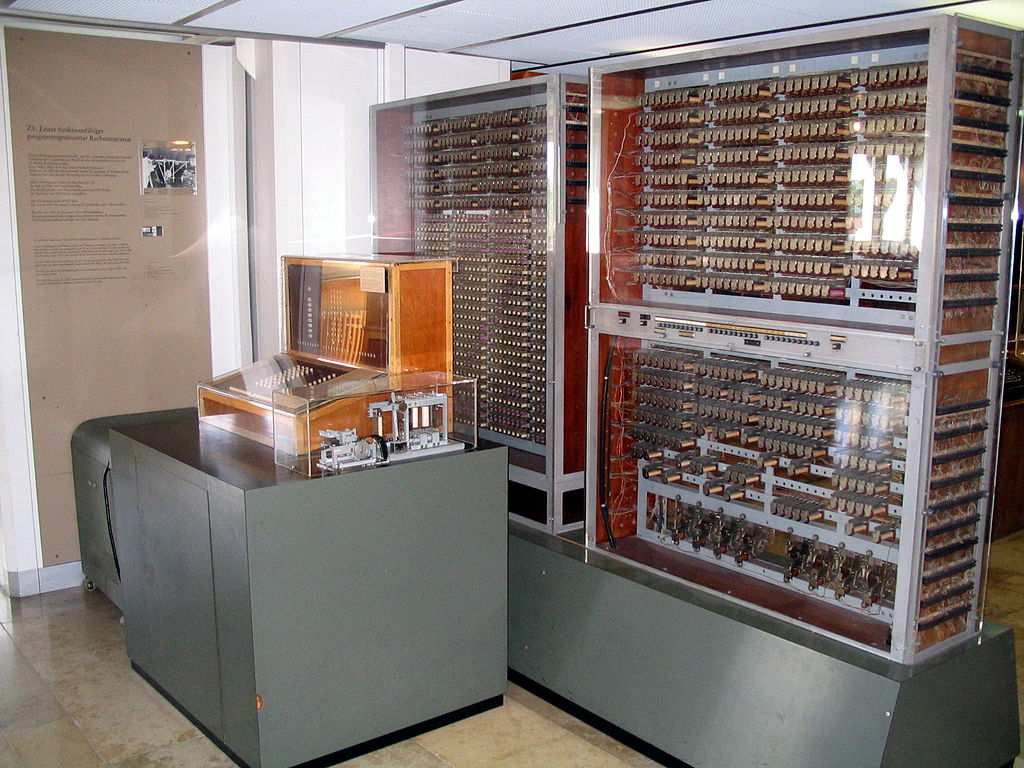
\includegraphics[width=6.4cm]{Z3_Deutsches_Museum.JPG}
	\end{minipage}
\end{frame}

\subsection{Tecnolg�a digital electr�nica}
\begin{frame}
	\frametitle{Atanasoff-Berry Computer}
	\begin{minipage}[c]{7.5cm}
		\begin{itemize}
			\item 1942
			\item Primera computadora electr�nica 
			\item Resoluci�n de equaciones diferenciales
			\item Mas de 300 tubos de vacio
			\item 2 DRUM de memoria capacitiva 1600 bits
			\item 30 operaciones por segundo
			\item 320 kg
		\end{itemize}
	\end{minipage}
	\begin{minipage}[c]{4cm}
		\begin{center}
			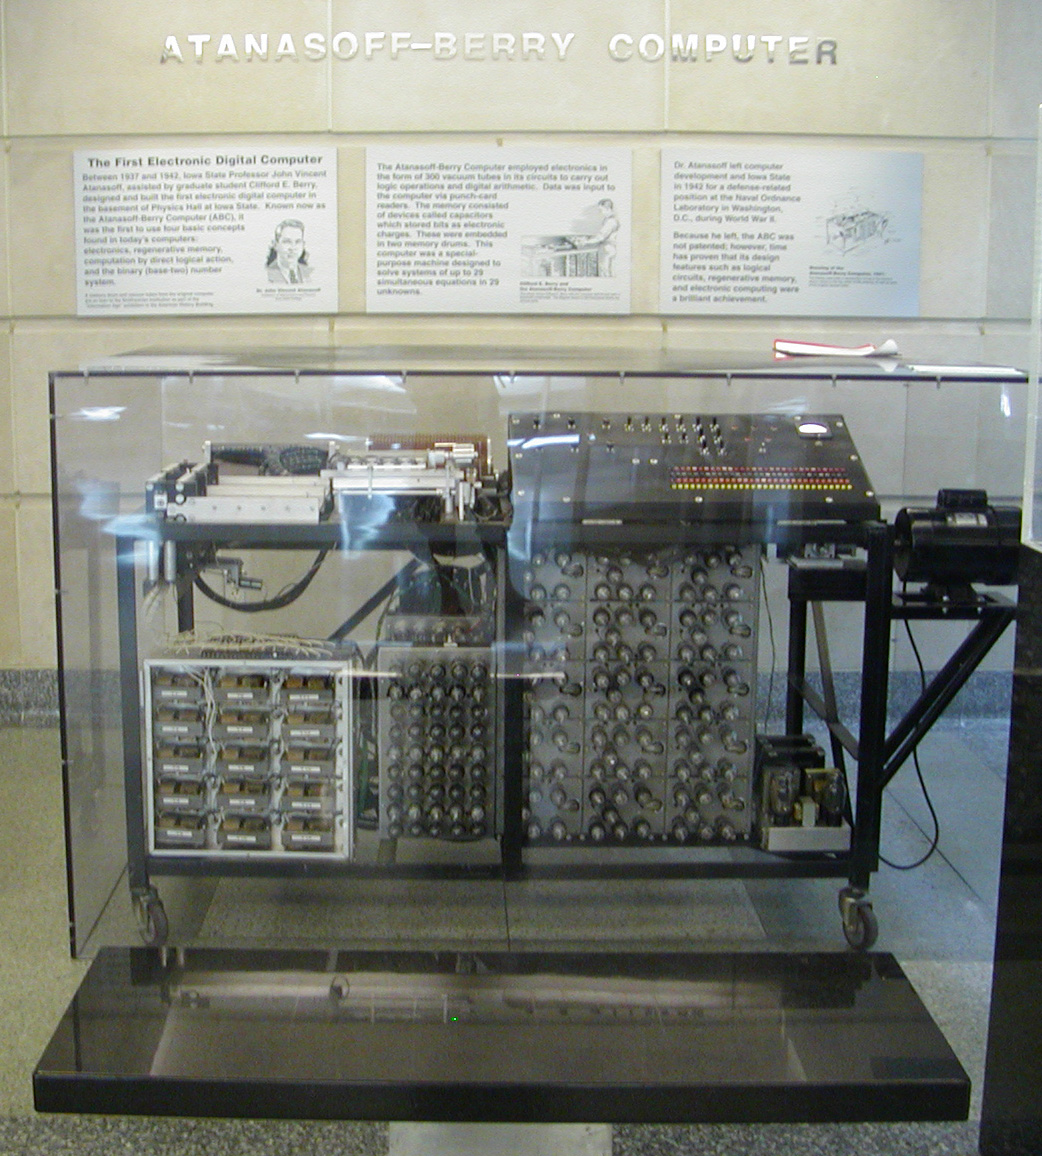
\includegraphics[width=4cm]{Atanasoff-Berry_Computer_at_Durhum_Center.jpg}
		\end{center}
	\end{minipage}
\end{frame}

\begin{frame}
\frametitle{Memoria Drum}
	\begin{minipage}[b]{7.5cm}
		\begin{itemize}
			\item 1932
			\item Gustav Tauschek
			\item Capacidad de 500 Kbits o 62.5 Kbytes
			\item Precursores de los HDD o discos rigidos
		\end{itemize}
	\end{minipage}
	\begin{minipage}[c]{4cm}
		\begin{center}
			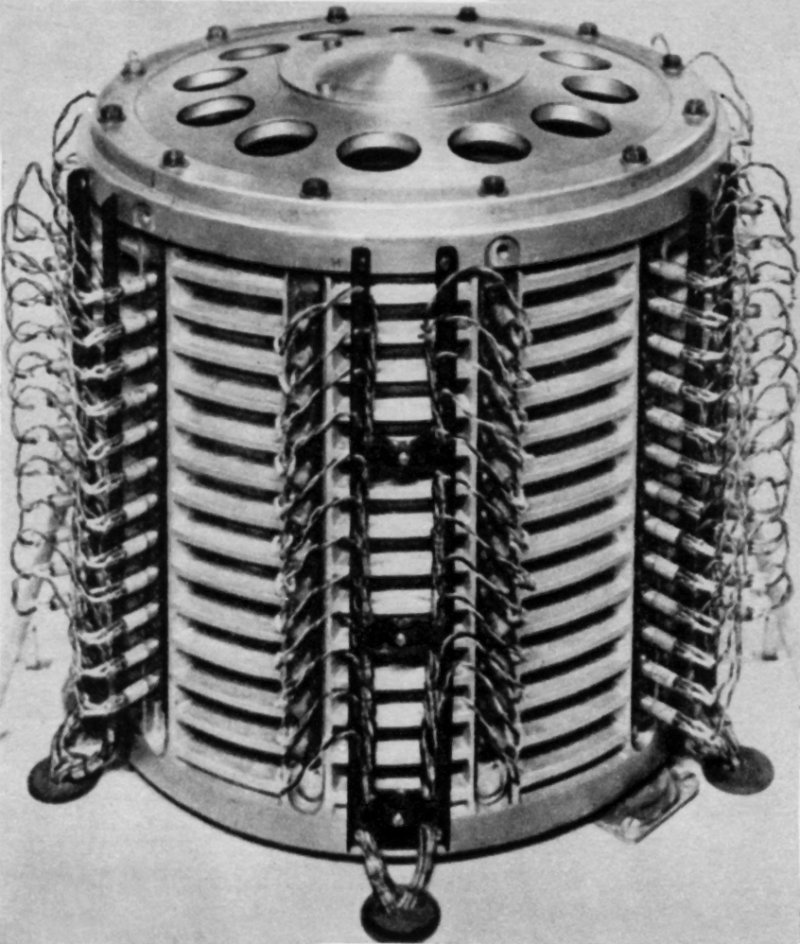
\includegraphics[height=4cm]{Pamiec_bebnowa_1.jpg}
		\end{center}
	\end{minipage}
\end{frame}

\begin{frame}
	\frametitle{Colossus}
	\begin{minipage}[c]{7.5cm}
	\begin{itemize}
		\item 1943
		\item Criptoan�lisis
		\item Programaci�n por interruptores y clavijas
		\item Mas de 1600 tubos de vacio
		\item Apodada Colosus por su tama�o.
	\end{itemize}
	\end{minipage}
	\begin{minipage}[c]{4cm}
		\begin{center}
			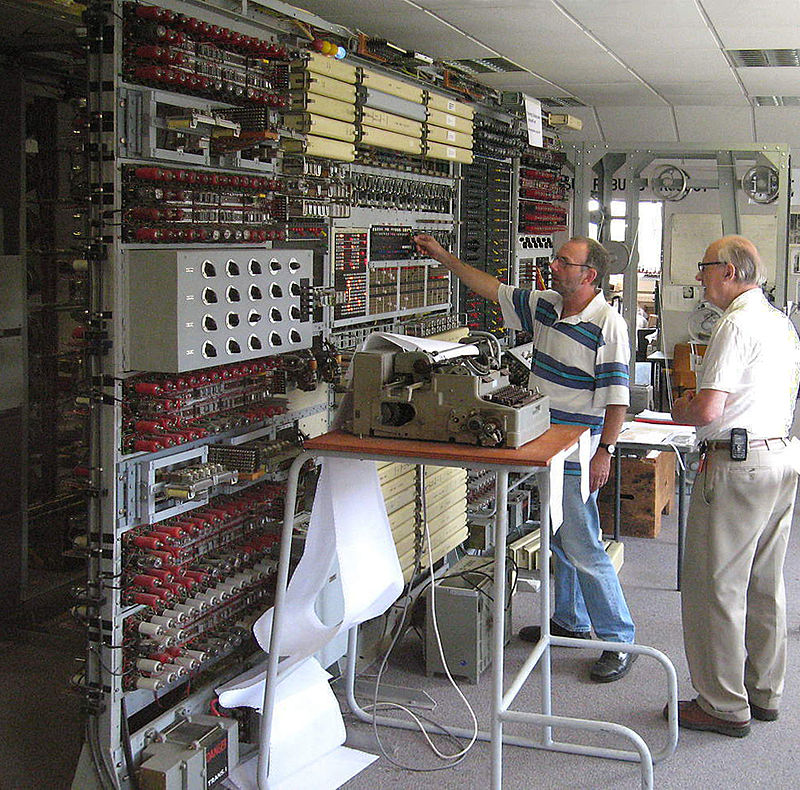
\includegraphics[width=4cm]{ColossusRebuild_11.jpg}
		\end{center}
	\end{minipage}
\end{frame}

\begin{frame}
\frametitle{ENIAC Electronic Numerical Integrator And Computer}
\framesubtitle{Descripci�n}
\begin{itemize}
	\item 1943
	\item C�lculo de trayectoria de misiles
	\item Programaci�n por interruptores y clavijas
	\item $10^{3}$ m�s r�pida en procesamiento que las electromec�nicas
	\item Memoria : 100 palabras de 10 digitos decimales o 4100 bits
	\item Recursos :
		\begin{itemize}
			\small
			\item 17.000 tubos de vacio
			\item 7.200 diodos de cristal
			\item 70.000 resistencias
			\item 10.000 capacitores
			\item 5.000.000 de soldaduras
			\item 150 KW
			\item 167 $m^{2}$
			\item 500.000 USD o 6.000.000 USD actualizados
		\end{itemize}
	\end{itemize}
\end{frame}

\begin{frame}
\frametitle{ENIAC o Electronic Numerical Integrator And Computer}
\begin{center}
	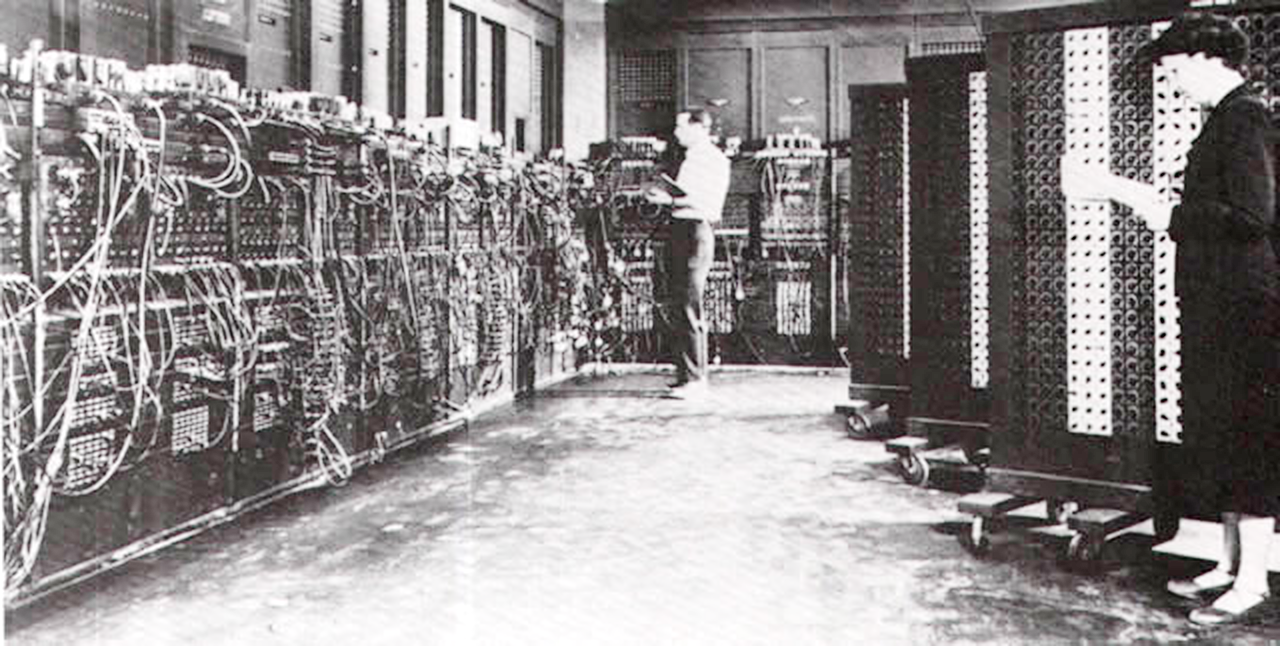
\includegraphics[width=11cm]{ENIAC.png}
\end{center}
\end{frame}

\begin{frame}
\frametitle{UNIVAC I UNIVersal Automatic Computer I}
	\begin{itemize}
		\item 1951-1954
		\item Proposito comercial
		\item Programaci�n en memoria
		\item 1.900 operaciones por segundo
		\item 1000 palabras de 11 digitos decimales
		\item Recursos
			\begin{itemize}
				\item 5.200 Tubos de vacio.
				\item Tecnolog�a de memoria Linea de Retardo de mercurio.
				\item 125 KW
				\item 13 toneladas
				\item 35.5 $m^{2}$
				\item Precio original 159.000 incrementandose hasta 1.500.000 USD
			\end{itemize}
	\end{itemize}
\end{frame}

\begin{frame}
	\frametitle{UNIVAC I (UNIVersal Automatic Computer I}
	\begin{center}
		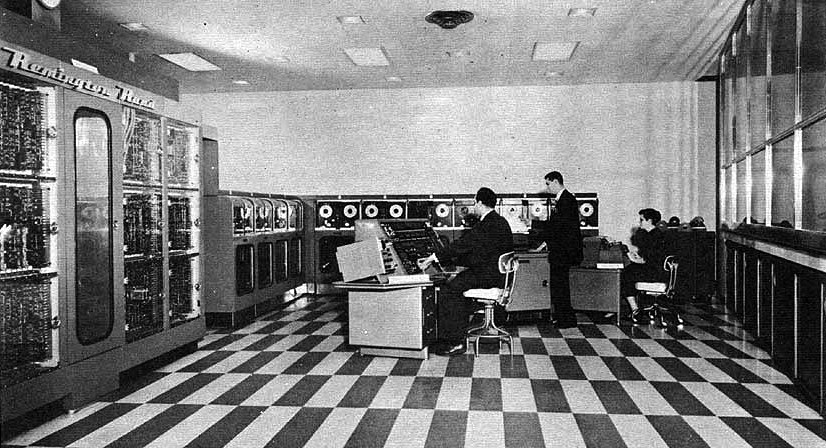
\includegraphics[width=11cm]{UNIVAC-I-BRL61-0977.jpg}
	\end{center}
\end{frame}

\begin{frame}
\frametitle{Memoria de linea de retardo}
\begin{minipage}[c]{7.5cm}
	\begin{itemize}
		\item 1947
		\item John Adam Presper Eckert
		\item Origen en las lineas de retardo para Radar
		\item EDVAC, UNIVAC I
		\item Medio de propagacion Mercurio
	\end{itemize}
\end{minipage}
\begin{minipage}[c]{4cm}
	\begin{center}
		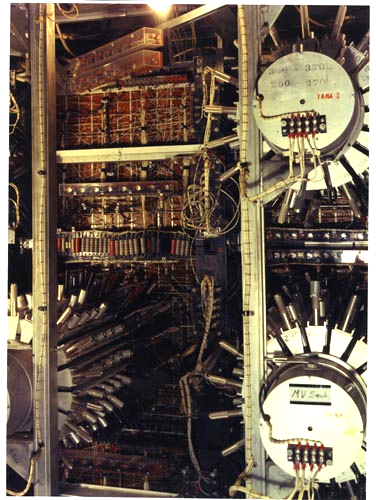
\includegraphics[width=4cm]{delay_line.png}
	\end{center}
\end{minipage}
\end{frame}

\subsection{Semiconductores}
\begin{frame}
\frametitle{}
	\begin{minipage}[c]{7.5cm}
		\begin{itemize}
			\item 1953 Universidad de Manchester
				\begin{itemize}
					\item 92-200 transistores
					\item 550-1300 diodos
					\item 150 Watts
				\end{itemize}
			\item 1954 Bell Labs TRADIC
			\item 1957 Calculadora IBM 608
		\end{itemize}
	\end{minipage}
	\begin{minipage}[c]{4cm}
		\begin{center}
			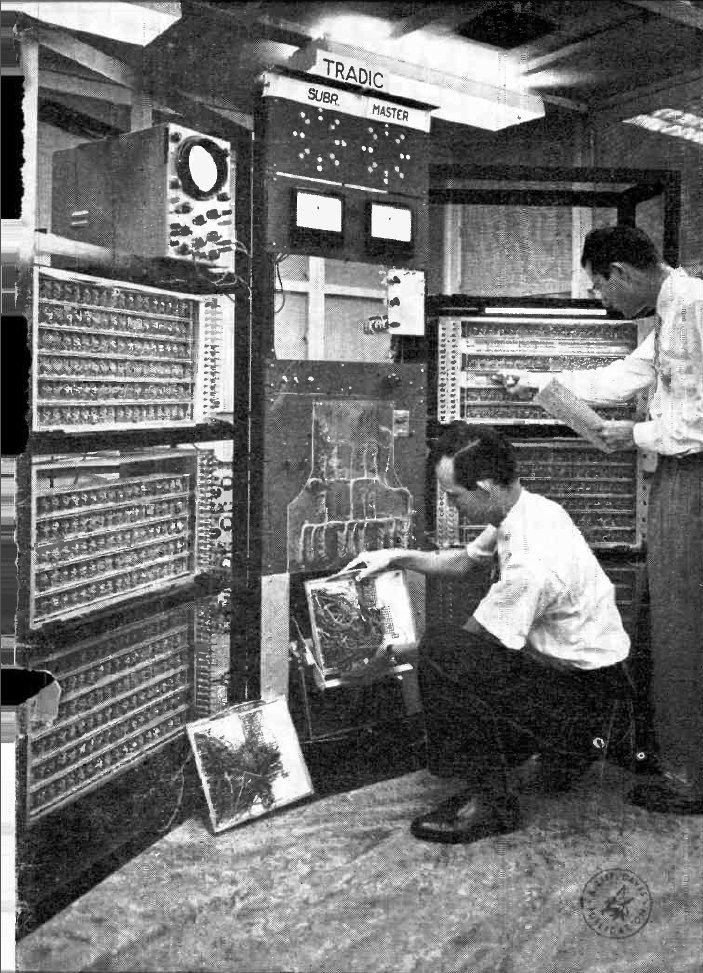
\includegraphics[width=4cm]{TRADIC_computer.jpg} \\ 
			Prototype TRADIC at Bell Labs, 1955. Felker is at left
		\end{center}
	\end{minipage}
\end{frame}

\begin{frame}
\frametitle{Compiladores}
	\begin{itemize}
		\item Principios de los 50s
		\item Programa generador autom�tico de c�digo de m�quina
		\item Ejemplos
			\begin{itemize}
				\item Autocode (principios de 1950)
				\item FLOW-MATIC (1955)
				\item FORTRAN (mediados de 1950)
				\item COBOL (1959)
				\item ALGOL (1960)
			\end{itemize}
	\end{itemize}
\end{frame}

\begin{frame}
\frametitle{Core memory}
	\begin{minipage}[c]{7.5cm}
		\begin{itemize}
			\item 1955-1975
			\item Toroides m�gneticos
			\item Lectura destructiva
			\item Costo de 1.00(1955) a 0.01(1975) USD por bit
			\item Tecnolog�as desplazadas
				\begin{itemize}
					\item DRUM
					\item Tubos de Vacio
					\item Transistores
				\end{itemize}
			\item Fabricadas por sastres en el este asi�tico
		\end{itemize}
	\end{minipage}
	\begin{minipage}[c]{4cm}
		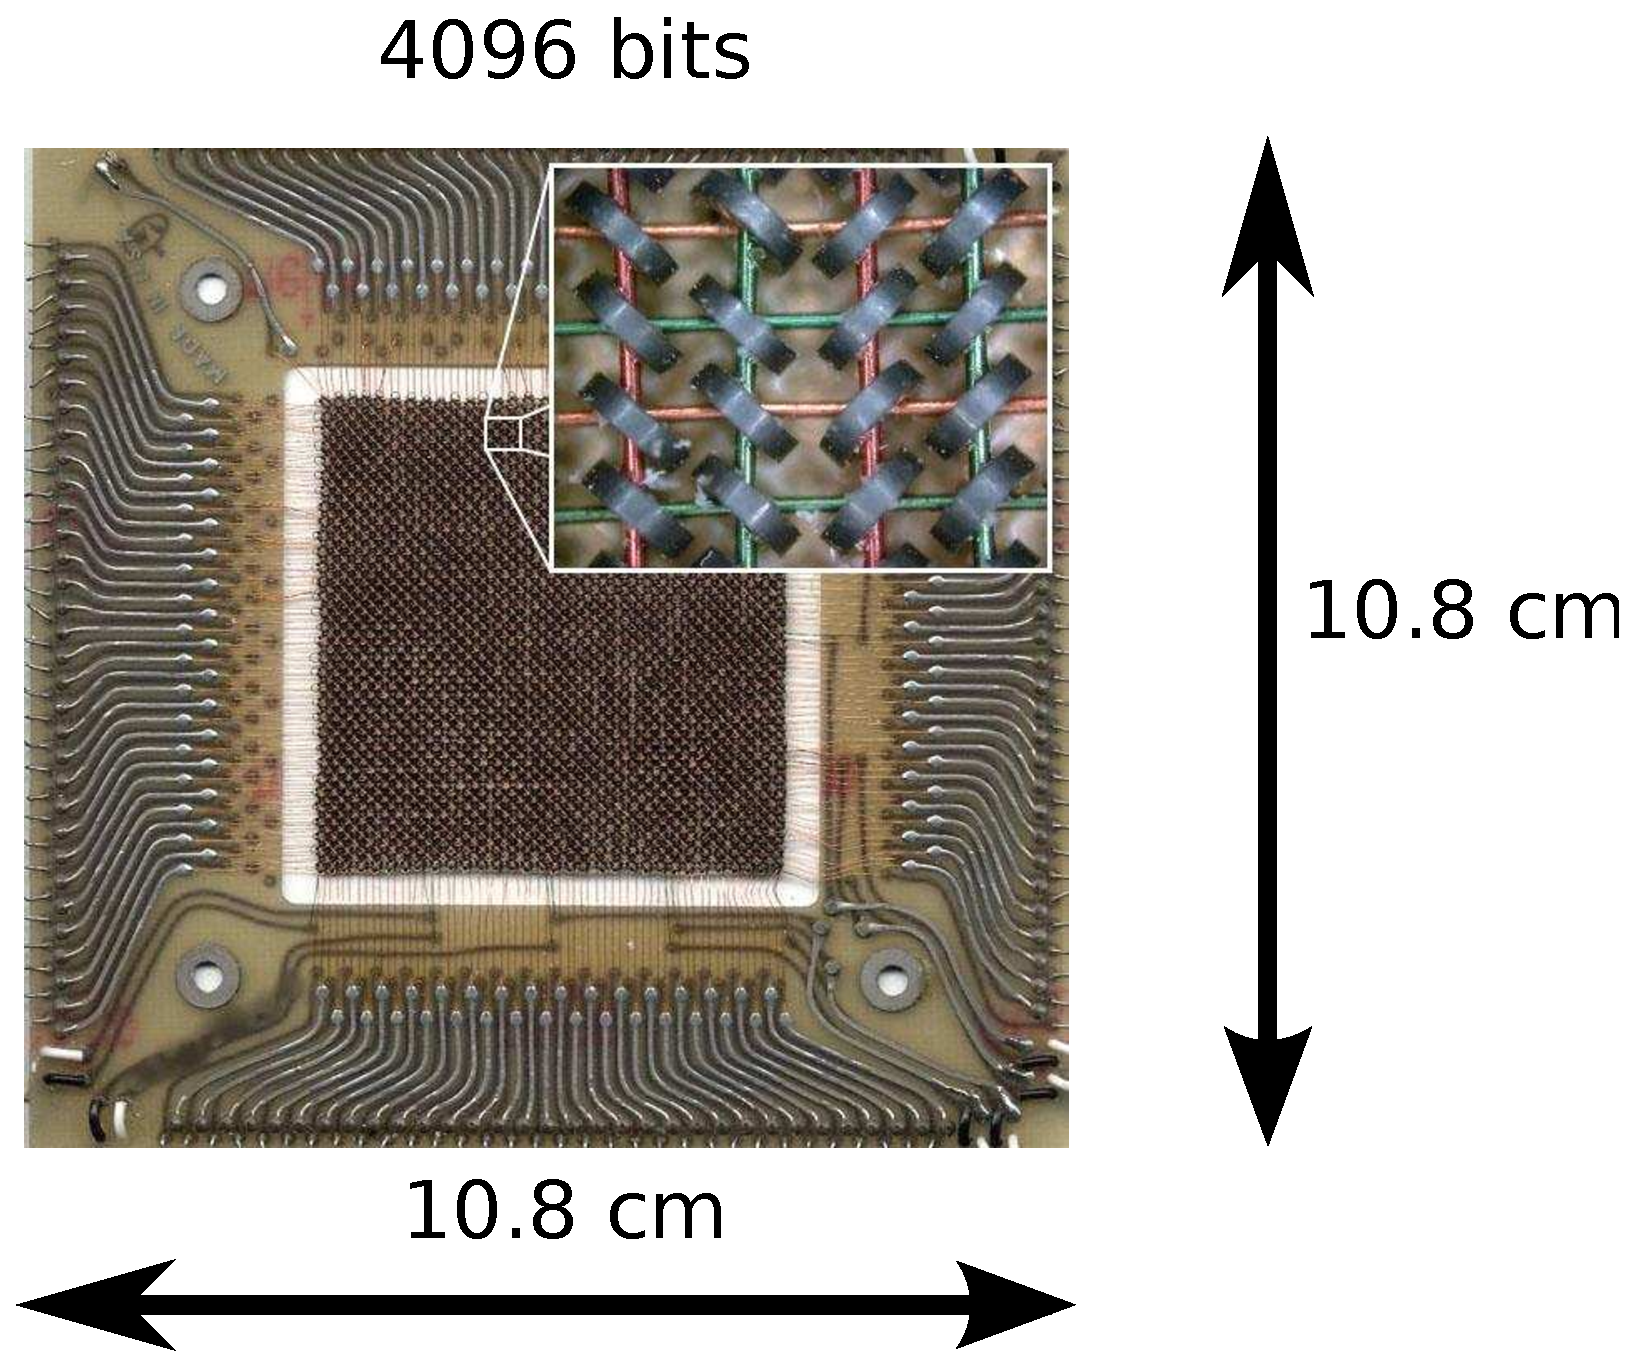
\includegraphics[width=4cm]{Ferrite_core_memory.eps} \\ \\
		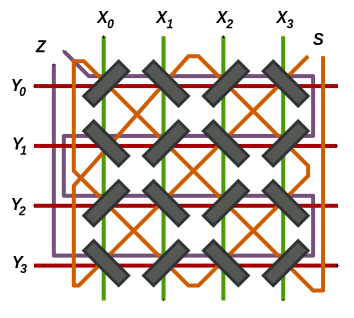
\includegraphics[width=2.5cm]{Coincident-current_magnetic_core.eps}
	\end{minipage}
\end{frame}

\begin{frame}
\frametitle{DRAM Memoria din�mica}
	\begin{minipage}[c]{4.5cm}
		\begin{center}
			\begin{itemize}
				\item 1966
				\item Robert Dennard
				\item Un transistor por bit
			\end{itemize}
		\end{center}
	\end{minipage}
	\begin{minipage}[c]{6.5cm}
		\begin{center}
		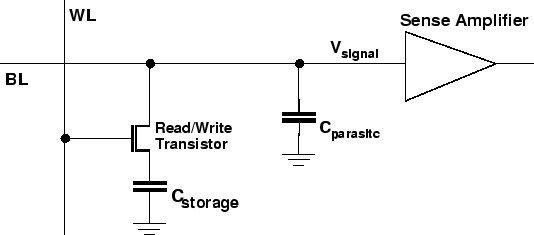
\includegraphics[width=6.5cm]{onetransistor.png} 
			%	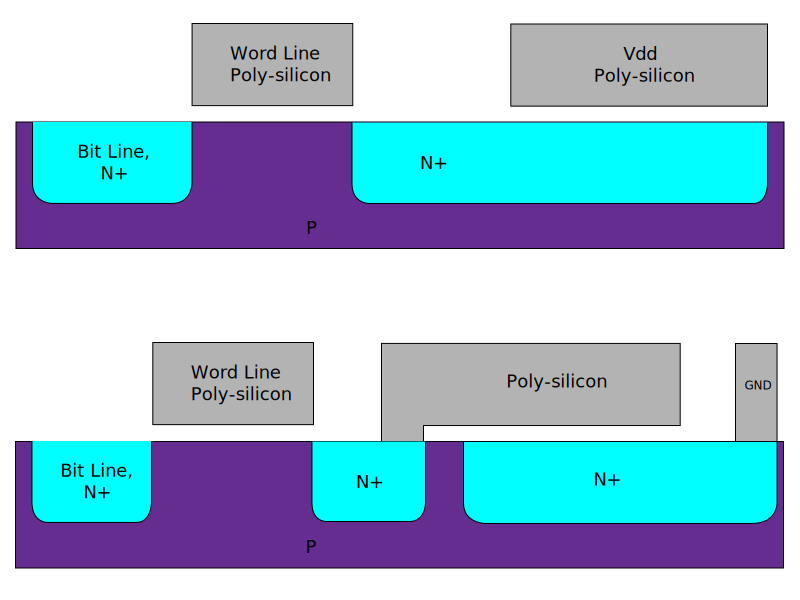
\includegraphics[width=5cm]{Original_1T1C_DRAM_design.eps}
		\end{center}
	\end{minipage}
\end{frame}

\begin{frame}
\frametitle{Multiplexado de la direcci�n}
	\begin{itemize}
		\item 1966-
		\item Robert Proebsting cofundador de Mostek
		\item Divide la direccion en dos y multiplexa las partes
			\begin{itemize}
				\item Filas \textbf{Row}
				\item Columnas \textbf{Column}
			\end{itemize}
		\item Reduce el tama�o del Chip y por consiguiente su costo.
		\item Fue ridiculizado por sus competidores.
		\item A finales del 70s dominaba el 85\% del mercado mundial.
	\end{itemize}
	\begin{center}
		\includegraphics[width=5cm]{MT4C1024-HD.jpg} 
		Memory Card with Integrated circuit Micron MT4C1024 1 Mbit DRAM chip. Die size 8662x3969 um.
	\end{center}
\end{frame}

\begin{frame}
\frametitle{Ley de Moore}
	\begin{itemize}
		\item 1975
		\item Gordon E. Moore Co-fundador de Intel
		\item Duplicacion de componentes por a�o en los circuitos integrados
	\end{itemize}
	\begin{center}
		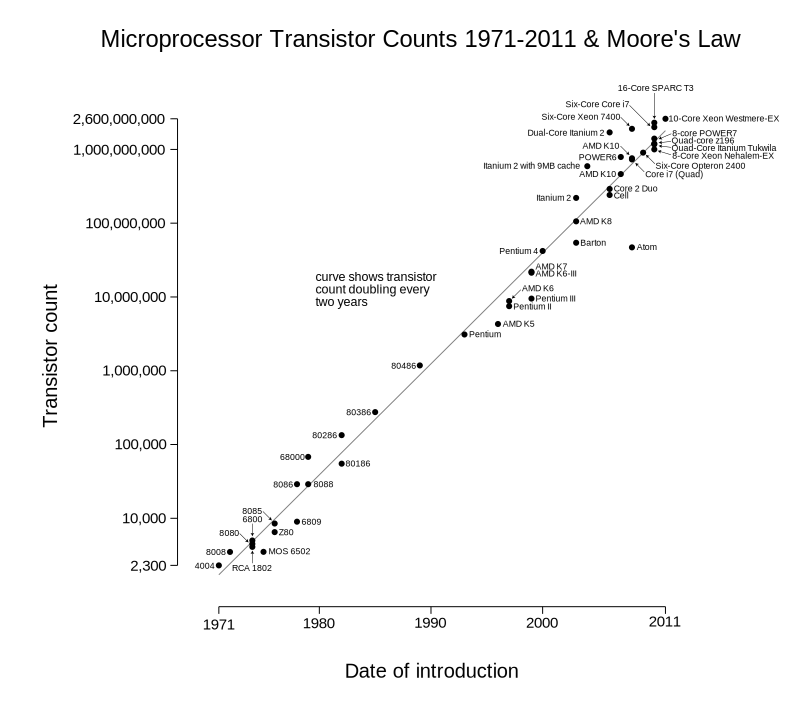
\includegraphics[width=7cm]{mooreslaw.eps} 
	\end{center}
\end{frame}

\begin{frame}
\frametitle{FPGAs Field Programmable Gate Arrays}
	\begin{itemize}
		\item 1985
		\item Arreglos de compuertas cuya red interconexi�n es programable.
		\item Depuraci�n de circutos digitales
	\end{itemize}
\end{frame}

\subsection{DRAM}
\begin{frame}
\frametitle{Banco de Memoria}
	\begin{center}
		\includegraphics[width=9cm]{membank.eps}
	\end{center}
\end{frame}

\begin{frame}
\frametitle{Lenguajes descriptores de hardware}
	\begin{itemize}
		\item Finales de los 60s
		\item Transferencia de Registros
	\end{itemize}
\end{frame}

\begin{frame}
\frametitle{Diagrama en Bloques}
	\begin{center}
		\includegraphics[width=10cm]{chip.eps}
	\end{center}
\end{frame}

\begin{frame}
\frametitle{Secuencia de acceso}
	\begin{itemize}
		\item Acceder a la fila con las lineas precargardas
		\item Conectar el amplificador de sensado
		\item Acceder a la columna
		\item Recuperar el valor leido
		\item Percargar las lineas a la mitad de la tension entre el 0 y el 1 logico
	\end{itemize}
\end{frame}

\subsection{Diagrama de tiempos}
\begin{frame}
	\begin{center}
		\includegraphics[width=11cm]{dram-timings.eps}
	\end{center}
\end{frame}

\begin{frame}
	\begin{center}
		\includegraphics[width=11cm]{sdrdram-timings.eps}
	\end{center}
\end{frame}

\begin{frame}
	\begin{center}
		\includegraphics[width=11cm]{ddrdram-timings.eps}
	\end{center}
\end{frame}

\section{fpga}
\begin{frame}
	\begin{center}
		\includegraphics[width=11cm]{fpga.eps}
	\end{center}
\end{frame}

\end{document}

